\section{Product forcing and support locality}\label{sec:forcing}

The monoid supplies copies of diagrams with controlled intersections.
We now turn those copies into two locality principles.  After the Cohen
generic is fixed, a diagram decides statements whose name parameters it
supports.  A value represented on two independent diagrams can then be
named on their common part.  These principles will classify quotients
and give the choice and coding properties needed to pass from quotients
to arbitrary sets.

\subsection{The choice ground and the two forcings}

The product separates the generic labels from their ground-model diagram
geometry. A related Cohen/tower product appears in
\cite[Section~3]{HolySchilhan2025}; the monoid and the diagram order used
here are specified below.

Work in a ground model \(V\) of \(\ZFC\).  Set
\[
 \kappa=\aleph_1^V,\qquad
 \mathfrak c=(2^{\aleph_0})^V,\qquad
 \mu=(\mathfrak c^+)^V,
 \qquad |I|^V=\mu^+.
\]
In the constructible ground used for the consistency result,
\(\mathfrak c=\aleph_1\), so these parameters are exactly
\(\kappa=\aleph_1\) and \(\mu=\kappa^+\).
The slightly more general choice of \(\mu\) will allow us to retain an
arbitrary given transitive choice ground.
All objects and cardinal calculations in the construction, unless
explicitly placed in an extension, belong to \(V\).

For every infinite cardinal \(\lambda<\mu\),
\[
 \lambda^{\aleph_0}\leq
 \mathfrak c^{\aleph_0}=\mathfrak c<\mu.
\]
Since \(\mu\) is regular and uncountable, every countable sequence in
\(\mu\) is bounded there.  It follows that
\begin{equation}\label{eq:ground-countable-arithmetic}
 \mu^{\aleph_0}=\mu.
\end{equation}
Take the monoid \(T\), with distinguished \(e\neq1\), from
Theorem~\ref{thm:monoid}, using this \(\mu\).
Let
\[
 \mathbb R=\operatorname{Add}(\kappa,I),\qquad
 \mathbb P=\{r:T\hookrightarrow I\},
 \qquad \mathbb Q=\mathbb R\times\mathbb P .
\]
Here a condition of \(\mathbb R\) is a partial function
\(I\times\kappa\to2\) with countable domain, ordered by reverse
inclusion.  Its coordinate support is
\[
 \supp_I(d)=
 \{j\in I:(\exists\alpha<\kappa)\ (j,\alpha)\in\dom(d)\}.
\]
For \(r\in\mathbb P\) and \(n\in T\), put
\[
 r_n(x)=r(nx),\qquad D_r=r[T],
 \qquad r\leq_{\mathbb P}s
       \ \Longleftrightarrow\
       (\exists n\in T)\ s=r_n .
\]
Thus a stronger diagram contains a specified copy of a weaker one.
The point \(r(1)\) is its center.  Whenever \(s=r_n\), the element
\(n\) is determined by the centers, since \(s(1)=r(n)\).
Left cancellation makes every \(r_n\) injective.  If
\(r=r_{nm}\), injectivity and conicality give \(n=m=1\); this
verifies antisymmetry of the order.  Transitivity follows from
\((r_n)_m=r_{nm}\).

The poset \(\mathbb P\) always denotes this \emph{ground} set,
including when it is forced over the Cohen extension.
No closure or cardinal-preservation assertion about \(\mathbb P\)
or the full product is needed.

\begin{lemma}\label{lem:cohen-properties}
The forcing \(\mathbb R\) is countably closed and satisfies the
\(\mu\)-chain condition.  It adds no countable sequences of ground
elements, preserves \(\kappa=\aleph_1^V\), and preserves every
ground cardinal at least \(\mu\).  In particular it preserves
\(\mu\) and \(\mu^+\).
If \(V\models\mathsf{CH}\), it preserves all cardinals.
\end{lemma}

\begin{proof}
A descending countable sequence has its union as a lower bound.
Deciding the entries of a name for a sequence in a ground set and
then taking such a lower bound shows that no new countable sequence
in that set is added.  This also preserves \(\omega_1^V\).

We recall the relevant delta-system argument to identify the exact
cardinal bound.  A family of \(\mu\) countable sets has a delta-system
subfamily of size \(\mu\).  Code its union into \(\mu\), and write
its members as \(S_\alpha\subseteq\mu\), for \(\alpha<\mu\).
There is a club of \(\delta<\mu\) such that
\(S_\alpha\subseteq\delta\) whenever \(\alpha<\delta\).
On the stationary part of this club of cofinality \(\omega_1\),
each \(S_\alpha\cap\alpha\) is bounded in \(\alpha\).
The pressing-down lemma makes a bound constant, say \(\gamma<\mu\),
on a stationary subset.  There are at most
\(|\gamma|^{\aleph_0}+\aleph_0<\mu\) possible countable subsets
of \(\gamma\), by
Equation~\eqref{eq:ground-countable-arithmetic} and its preceding
bound.  Regularity of \(\mu\) therefore makes
\(S_\alpha\cap\alpha\) one fixed set on a stationary subset.
For \(\alpha<\beta\) in that subset,
\(S_\alpha\subseteq\beta\), so their intersection is this fixed root.

Apply this to the domains of \(\mu\) Cohen conditions.
There are at most \(2^{\aleph_0}=\mathfrak c<\mu\)
assignments on the countable root.  Thinning once more gives two,
indeed \(\mu\), conditions agreeing on the root.  They are compatible,
which proves the chain condition.
The usual antichain bound then preserves all cardinals at least
\(\mu\): the possible values at any one coordinate of a name for
an ordinal-valued function are covered by fewer than \(\mu\)
ground ordinals, and regularity handles the case of \(\mu\) itself.
Countable closure and the chain condition together preserve all
cardinals when \(\mu=\aleph_2\).
In a general ground we assert no preservation of cardinals strictly
between \(\kappa\) and \(\mu\).

Finally, any sequence of ground elements has its values in some ground
rank segment: their ranks have an ordinal bound, and forcing preserves
ordinals.  Thus the assertion about sequences in ground sets covers
all countable sequences of ground elements.
\end{proof}

\begin{lemma}[Extending and amalgamating diagrams]
\label{lem:diagram-amalgamation}
\begin{enumerate}
\item
For every \(p\in\mathbb P\) and ground \(J\subseteq I\) of size at
most \(\mu\), there is \(r\in\mathbb P\) with
\(r_e=p\) and \(J\subseteq D_r\).
\item
A finite family \(s_i\in\mathbb P\) has a common extension whenever
each pair has either disjoint ranges or an intersection that is
exactly the range of a common subdiagram
\[
 s_{i,a_{ij}}=s_{j,a_{ji}}.
\]
\item
A partial placement of finitely many diagrams that is injective and
consistent on their
specified common parts, extends to a ground permutation of \(I\).
Unspecified coordinates of these diagrams and of finitely many Cohen
conditions can be placed outside any prescribed ground set of size
at most \(\mu\).
\end{enumerate}
\end{lemma}

\begin{proof}
The probes from Theorem~\ref{thm:monoid} for
\(a=1,b=e,U=\{1\}\) give \(\mu\) distinct elements \(m\) with
\(me=e\).  None belongs to \(eT\): if \(m=ex\), left cancellation
would give \(xe=1\), contrary to conicality and \(e\neq1\).
Hence \(|T\setminus eT|=\mu\).
Define \(r(ex)=p(x)\), using left cancellation, and fill the
complement injectively in \(I\setminus D_p\), including
\(J\setminus D_p\).  Both the size of that complement in \(T\)
and the strict inequality \(\mu<|I|\) give the first assertion.

For the second assertion, identify the copies of \(T\) exactly where
their labels in \(I\) coincide.  The hypothesis says that these
identifications have the form required by the finite-merger property;
their transitivity and absence of collapse within a copy follow from
actual equality of labels.  Let \(l_i\in T\) realize this merger.
On \(\bigcup_i l_iT\), assign \(l_ix\) the value \(s_i(x)\).
The exact-overlap property makes this well defined and injective.
Extend it injectively to the rest of \(T\).  The resulting \(r\)
satisfies \(r_{l_i}=s_i\).

For the last assertion, the prescribed domain and range each have
size at most \(\mu\).  Their complements in \(I\) both have
cardinality \(\mu^+\), so a bijection between the complements
extends the partial bijection to a permutation.
Fresh images can first be chosen off the excluded set, whose size
is still at most \(\mu\), and then the same argument applies.
All these choices occur in \(V\).
\end{proof}

\subsection{The symmetric system and transport}

Let \(G=\Sym(I)^V\).  A permutation acts simultaneously on diagrams
and on Cohen coordinates:
\[
 (\pi r)(x)=\pi(r(x)),\qquad
 (\pi d)(\pi j,\alpha)=d(j,\alpha).
\]
These are automorphisms of \(\mathbb Q\).
For ground \(J\subseteq I\), let \(\Fix(J)\) be its pointwise
stabilizer in \(G\), and set
\[
 \mathcal F=
 \{K\leq G:(\exists J\in V)\,
       [J\subseteq I,\ |J|^V\leq\mu,\ \Fix(J)\subseteq K]\}.
\]
This is a normal filter of subgroups.
Finite intersections are handled by \(J\cup J'\), and
\(\pi\Fix(J)\pi^{-1}=\Fix(\pi J)\).

The action on names is recursive:
\[
 \pi\tau=\{(\pi\sigma,\pi u):(\sigma,u)\in\tau\}.
\]
A name has support \(J\) when \(\Fix(J)\) fixes it literally.
A hereditarily symmetric name, abbreviated \(\HS\), has a support
and only hereditarily symmetric member names.
There is no restriction on name rank.
Ground check names are fixed by every permutation.
Canonical ordered-pair and sequence names commute with the action.
When the poset has no largest condition, their usual definitions use
all conditions in place of that condition; equivalently one may
adjoin a fixed largest condition.

For the evaluated presentation, assume that \(V\) is externally
transitive and that the indicated generic filters are available in the
ambient universe.  Over a general choice ground, the same construction
and the generic notation below express internal forcing assertions;
they do not require external recursion on its membership relation.
Section~\ref{sec:metatheory} realizes these assertions over an arbitrary
countable ground by a quotient of internal names.

Write \(F\) for an \(\mathbb R\)-generic filter over \(V\), and
\(H\) for a generic on the ground \(\mathbb P\) over \(V[F]\).
The product extension is \(V[F][H]\).  A product name \(\tau\),
after evaluating its Cohen part, becomes a \(\mathbb P\)-name
denoted by \(\tau[F]\).
Let
\[
 W=\{\tau^{F\times H}:\tau\in\HS^V\}.
\]

\begin{theorem}[The symmetric-model theorem]\label{thm:symmetric-model}
The symmetric forcing relation is definable formula by formula in
\(V\), and it forces every axiom instance of full pure-set \(\ZF\).
If \(V\) is externally transitive, the evaluated class \(W\) is
a transitive model of that theory, with
\[
 V\subseteq W\subseteq V[F][H],
 \qquad \Ord^W=\Ord^{V[F][H]}.
\]
The truth lemma holds for this evaluated model.  Over an arbitrary
countable choice ground, it holds for the symmetric quotient of internal
names described in Section~\ref{sec:metatheory}.
\end{theorem}

\begin{proof}
Apply the set-forcing symmetric-extension theorem
\cite[Section~2.1, p.~4]{Karagila2026} to \(\mathbb Q\), \(G\),
and the normal subgroup filter verified above.
Its internal formulation concerns all hereditarily symmetric names
and yields the full Separation and Replacement schemata, as well as
Foundation; this formulation is recalled in
Lemma~\ref{lem:symmetric-forcing-schema}.  It requires no
countable-completeness assumption on the filter.  External transitivity
of \(V\) permits the usual recursive name evaluation and gives the
displayed literal inclusions.  For an arbitrary countable ground,
Lemma~\ref{lem:arbitrary-model-symmetric-truth} instead gives truth
in the membership-closed symmetric quotient; it makes no assertion
of external well-foundedness.
\end{proof}

The generic terminology below expresses arguments with the ordinary
and symmetric forcing relations.  In particular, each assertion about
all generics can instead be read as its forcing-theoretic assertion
over the choice ground.  The formal consistency deduction is given
after the construction.

We will use symmetry in its precise product form:
\begin{equation}\label{eq:product-symmetry}
 (d,s)\forces_{\mathbb Q}\varphi(\vec\tau)
 \quad\Longleftrightarrow\quad
 (\pi d,\pi s)\forces_{\mathbb Q}\varphi(\pi\vec\tau).
\end{equation}
The corresponding evaluation identity is
\[
 (\pi\tau)^{\pi F\times\pi H}=\tau^{F\times H}.
\]
It does not define an automorphism of one fixed extension by sending
\(\tau^{F\times H}\) to \((\pi\tau)^{F\times H}\).
The product/iteration equivalence also gives the factorized version
of Equation~\eqref{eq:product-symmetry}: a Cohen condition forcing
\(s\forces_{\mathbb P}\varphi(\vec\tau[F])\) is transported to a
Cohen condition forcing the corresponding assertion at \(\pi s\)
with names \(\pi\vec\tau\).
Here \(\pi s\) is explicitly reindexed ground data; it is not the
image of \(\check s\) under the name action, which fixes check names.

Let \(\dot A_j\) be the canonical name for the Cohen subset of
\(\kappa\) at coordinate \(j\), and put
\[
 A_j=\dot A_j^{F\times H},\qquad A=\{A_j:j\in I\}.
\]
The name \(\dot A_j\) has support \(\{j\}\), and
\(\pi\dot A_j=\dot A_{\pi j}\).
The name for \(A\) is invariant.  Distinct coordinates give distinct
labels: below any Cohen condition, assign different bits at one
ordinal unused at the two coordinates.  This proves forced
distinctness, which persists after the second forcing.

\subsection{Decision and descent}

Restriction to supporting coordinates and descent to a common support
have precedents in \cite[Lemmas~10 and~15]{HolySchilhan2025}.
The following proofs establish the versions needed for our diagrams,
including arbitrary-rank product names and exact compatibility of the
moved conditions.

The two factors play different roles in the first lemma.  Once the
Cohen generic is fixed, strengthening a supporting diagram cannot change
the truth of a supported assertion.  The assertion can still depend on
the Cohen generic; the second part says that a Cohen condition witnessing
it may discard coordinates outside the supporting diagram.

\begin{lemma}[Decision over a supporting diagram]
\label{lem:local-decision}
Fix an \(\mathbb R\)-generic \(F\).
\begin{enumerate}
\item
If \(p\in\mathbb P\) and all product-name parameters
\(\tau_1,\ldots,\tau_k\) are supported by \(D_p\), then \(p\)
decides each ordinary \(\mathbb P\)-forcing formula
\(\varphi(\tau_1[F],\ldots,\tau_k[F])\) in \(V[F]\).
The parameters may have arbitrary rank.
\item
Suppose a Cohen condition \(d\) forces that
\(s\forces_{\mathbb P}\varphi(\vec\tau[F])\), where all the
product names are supported by \(D_s\).
Then \(d\restriction(D_s\times\kappa)\) forces the same assertion.
\end{enumerate}
For brevity we write \(d\restriction D_s\) for this restriction.
\end{lemma}

\begin{proof}
If the first assertion fails, there are \(s_0,s_1\leq p\)
forcing contrary answers in \(V[F]\).
Choose \(d_0,d_1\in F\) witnessing those answers in the factorized
forcing relation.  Their restrictions to \(D_p\times\kappa\)
are compatible.
By Lemma~\ref{lem:diagram-amalgamation}, choose
\(\pi\in\Fix(D_p)\) so that, outside \(D_p\), the coordinates
of \(s_1,d_1\) move away from those of \(s_0,d_0\).
The diagrams \(s_0,\pi s_1\) meet exactly in their common
subdiagram \(p\), so have a common extension.
The conditions \(d_0,\pi d_1\) agree on the root and have
disjoint supports off it, so are compatible.
All parameter names are fixed by \(\pi\).
Equation~\eqref{eq:product-symmetry} now gives two contrary assertions
forced by compatible product conditions, a contradiction.
This argument does not assert that \(\pi d_1\) belongs to \(F\).

For the second assertion, put \(\delta=d\restriction D_s\).
If \(\delta\) does not force the indicated factorized assertion,
there is \(c\leq\delta\) forcing its negation.
Choose \(\pi\in\Fix(D_s)\) moving
\(\supp_I(d)\setminus D_s\) off \(\supp_I(c)\setminus D_s\).
The condition \(\pi d\) is compatible with \(c\).
It forces the original factorized assertion, by product symmetry,
because \(s\) and all its parameter names are fixed.
This contradicts the assertion forced by \(c\).
\end{proof}

We next show that equality between independently supported values
can be represented on the intersection.  The proof uses a third copy
to compare the two values while keeping an arbitrary potential
counterexample compatible.

\begin{lemma}[Support descent]\label{lem:support-descent}
Suppose \(s_0,s_1\leq p\) and
\(D_{s_0}\cap D_{s_1}=D_p\).
Let \(\sigma_i\) be product \(\HS\) names supported by \(D_{s_i}\).
Fix an \(\mathbb R\)-generic \(F\).
If some \(v\leq s_0,s_1\) forces
\(\sigma_0[F]=\sigma_1[F]\) in ordinary \(\mathbb P\)-forcing,
then there is a product \(\HS\) name \(\sigma\), supported by
\(D_p\), such that
\[
 s_i\forces_{\mathbb P}\sigma[F]=\sigma_i[F]
 \qquad(i=0,1)
\]
in \(V[F]\).
The names may have arbitrary rank.
If, in \(V[F]\), each \(s_i\) also forces
\(\sigma_i[F]\subseteq A\), the descended name can be normalized
to a subset name with only label names as possible members.
\end{lemma}

\begin{proof}
Take \(d\in F\) witnessing the equality forced at \(v\).
Both parameter supports lie in \(D_v\), so
Lemma~\ref{lem:local-decision} allows us to replace \(d\) by
\(d\restriction D_v\).  Set
\(\delta=d\restriction D_{s_0}\).
We will combine the translates of \(\sigma_0\) into one
\(D_p\)-supported name.  A translate contributes its value only when
the generic contains the corresponding translate of
\((\delta,s_0)\); the value of the new name will be the union of these
contributing values.  Thus the main task is to prove that any two
contributing copies agree.  For this coherence argument, allow both
factors of the product generic to vary.  We will return to the fixed
\(F\) after constructing the name.

For every \(\pi\in\Fix(D_p)\), call the copy
\(\pi\sigma_0\) \emph{active} when its trigger
\((\pi\delta,\pi s_0)\) belongs to the product generic.
We first prove that any two active copies have equal values.

Consider two copies whose diagrams \(\bar s,\bar s'\) have
intersection exactly \(D_p\).  If they can be unequal while active,
some product condition \((c,t)\) extends both triggers and forces
the inequality.
Place a copy \(u\) of \(s_1\) over \(p\), with the rest of its
range fresh relative to \(D_t\cup\supp_I(c)\).
Extend the respective placements of
\((s_0,s_1)\) onto \((\bar s,u)\) and \((\bar s',u)\) to
placements of \(v\), producing diagrams \(v',v''\).
Use the same placement on all of \(D_{s_1}\) in both cases.
Choose all remaining coordinates freshly, so that the ranges have the
intersections shown in Figure~\ref{fig:support-descent}:
\begin{equation}\label{eq:descent-three-overlaps}
 \begin{aligned}
 D_{v'}\cap D_t&=D_{\bar s},&
 D_{v''}\cap D_t&=D_{\bar s'},&
 D_{v'}\cap D_{v''}&=D_u .
 \end{aligned}
\end{equation}
\begin{figure}[htbp]
\centering
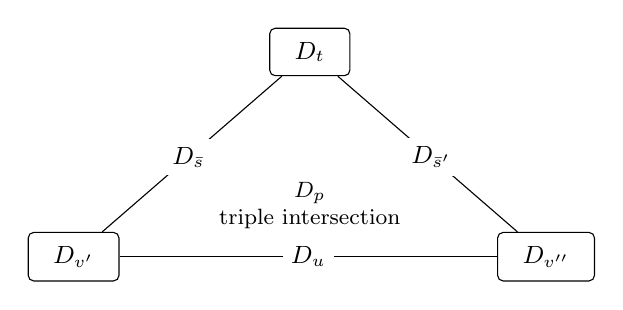
\begin{tikzpicture}[font=\small,
    diagramrange/.style={draw,rounded corners=2pt,fill=white,
                  inner xsep=9pt,inner ysep=5pt},
    overlap/.style={fill=white,inner sep=3pt}]
  \node[diagramrange] (t) at (0,1.8) {$D_t$};
  \node[diagramrange] (v) at (-3,-.8) {$D_{v'}$};
  \node[diagramrange] (w) at (3,-.8) {$D_{v''}$};
  \draw (t) -- node[overlap,pos=.52] {$D_{\bar s}$} (v);
  \draw (t) -- node[overlap,pos=.52] {$D_{\bar s'}$} (w);
  \draw (v) -- node[overlap] {$D_u$} (w);
  \node[align=center,font=\footnotesize] at (0,-.15)
    {$D_p$\\triple intersection};
\end{tikzpicture}
\caption{The independent-copy case of support descent. Each edge is
labelled by the exact intersection of its endpoint ranges. The two
placed equality witnesses $v',v''$ use the same fresh copy $u$ of $s_1$;
$t$ carries the proposed inequality between the copies on
$\bar s$ and $\bar s'$, whose ranges meet exactly in $D_p$.
These exact intersections allow the three diagrams to be amalgamated
over their common root $p$.}
\label{fig:support-descent}
\end{figure}

Every intersection in this display is its indicated common
subdiagram.  The required partial maps agree on the root, and
their domain and range sizes are at most \(\mu\);
Lemma~\ref{lem:diagram-amalgamation} therefore supplies the
ground permutations realizing these placements.

The two placed copies of \(d\) agree on \(D_u\).
They agree with \(c\) on \(D_{\bar s}\) and \(D_{\bar s'}\),
respectively, because \(c\) extends the two placed copies of
\(\delta\).  On the remaining coordinates freshness gives
compatibility.  Thus the Cohen conditions have a common extension.
The three diagrams \(v',v'',t\) also have a common extension by
Equation~\eqref{eq:descent-three-overlaps} and finite amalgamation.
The two transported \(\sigma_1\) names are literally equal,
since the placements agree on the entire \(D_{s_1}\).
The equalities transported from \((d,v)\) therefore contradict
the inequality forced by \((c,t)\).

For two active copies with arbitrary overlap, start again with
any proposed inequality-forcing common extension \((c,t)\).
Place a third copy of \(s_0\) over \(p\), independent of \(t\)
off the root, and place its Cohen trigger compatibly with \(c\).
It has a common product extension with \((c,t)\).
The independent case just proved applies between this third copy
and each of the original ones, contradicting the inequality.
This proves coherence of all active copies, below every possible
inequality witness.

Define a mixture using all joint strengthenings:
\begin{equation}\label{eq:descent-mixture}
 \sigma=
 \left\{(\pi\eta,(c,t)):
 \begin{array}{l}
 \pi\in\Fix(D_p),\quad (\eta,(a,u))\in\sigma_0,\\
 (c,t)\leq(\pi\delta,\pi s_0),\quad
 (c,t)\leq(\pi a,\pi u)
 \end{array}\right\}.
\end{equation}
This is a set name.
Left multiplication in \(\Fix(D_p)\) permutes its entries, so it
is supported by \(D_p\).
Its member names are translates of member names of \(\sigma_0\)
and hence are \(\HS\).
In any product generic its value is the union of the values of
the active copies.  Both inclusions in this description follow
from directedness of the generic: all common strengthenings,
rather than a selected one, occur in
Equation~\eqref{eq:descent-mixture}.
When the original trigger is active, coherence makes this union
exactly the value of \(\sigma_0\).
Return now to the fixed \(F\).  Since \(\delta\in F\), the
original trigger is active in every product generic with this Cohen
factor and with \(s_0\) in its diagram filter.  It follows that
\(s_0\forces_{\mathbb P}\sigma[F]=\sigma_0[F]\).
The equality with \(\sigma_1[F]\) holds below \(v\).
Its parameters are supported by \(D_{s_1}\), so
Lemma~\ref{lem:local-decision} makes it hold already below \(s_1\).

No step imposed a rank bound.
For the subset assertion, replace the mixture by its intersection
with \(A\), using the normalization in the next paragraph.
\end{proof}

For \(r\in\mathbb P\), define the following ground set of names:
\begin{equation}\label{eq:normalized-local-names}
 \mathcal X(r)=
 \left\{\tau\subseteq
     \{\dot A_j:j\in I\}\times\mathbb Q:
       (\forall\pi\in\Fix(D_r))\ \pi\tau=\tau\right\}.
\end{equation}
Every member is \(\HS\).
If a product \(\HS\) name \(\tau\) is supported by \(J\), define
\[
 \tau\mathbin{\upharpoonright} A=
 \{(\dot A_j,u):j\in I,\ u\in\mathbb Q,\
                         u\forces_{\mathbb Q}\dot A_j\in\tau\}.
\]
The ordinary truth lemma gives value \(\tau^{F\times H}\cap A\).
Symmetry preserves the support \(J\).
In particular a name supported by \(D_r\) whose actual value is
a subset of \(A\) has the same value as some member of
\(\mathcal X(r)\).
This is a set-sized normalization, valid for an original name of
any rank.

\subsection{Coding arbitrary sets by the labels}

The next argument extracts a partial function from an orbit of a name.
The diagram condition in the function's definition ensures that equal
inputs have equal values.

\begin{proposition}\label{prop:presentation}
In \(W\), every nonempty set \(X\) is the image of a surjection
\(A\times\eta\to X\) for some ordinal \(\eta\).
No bound on the rank of \(X\) is imposed.
\end{proposition}

\begin{proof}
Let \(\sigma\) be a ground \(\HS\) name, and let \(p\) have
\(D_p\) as a support for \(\sigma\).
Form the graph name
\begin{equation}\label{eq:partial-orbit-map}
 \dot h_{\sigma,p}=
 \left\{\left(
    \operatorname{op}(\dot A_{\pi(p(1))},\pi\sigma),
                      (1_{\mathbb R},\pi p)\right):\pi\in G\right\},
\end{equation}
where \(\operatorname{op}\) denotes the canonical ordered-pair name.
This name is invariant, and all its member names are \(\HS\).

Its value is a partial function on \(A\).
Indeed, suppose two contributing pairs have equal first coordinates.
Label distinctness gives
\(\pi(p(1))=\rho(p(1))\).
There is a common extension \(r\in H\) of \(\pi p,\rho p\);
write \(\pi p=r_n\) and \(\rho p=r_m\).
The equality of centers and injectivity of \(r\) give \(n=m\).
Consequently \(\pi p=\rho p\) pointwise, so
\(\rho^{-1}\pi\in\Fix(D_p)\).
It fixes \(\sigma\), and hence \(\pi\sigma=\rho\sigma\)
literally.  The two values therefore agree.
This argument concerns names under compatible diagram conditions,
not an action on one fixed symmetric model.

The orbit construction gives invariant partial functions.  We now
form a set-indexed family of them whose ranges cover \(X\).
Choose an \(\HS\) name \(\tau\) for \(X\).
The set \(M\) of member names appearing in \(\tau\) is a ground
set of \(\HS\) names.  In \(V\), enumerate by an ordinal \(\eta\)
the set
\[
 B=\{(\sigma,p)\in M\times\mathbb P:
                         \Fix(D_p)\text{ fixes }\sigma\}.
\]
Every member name has a support of size at most \(\mu\), and
Lemma~\ref{lem:diagram-amalgamation} provides supporting diagrams.
We include all such diagrams, because one chosen diagram need not
belong to the generic filter.
The corresponding sequence of graph names
\(\dot h_{\sigma,p}\) is a ground sequence of invariant
\(\HS\) names.  Its canonical sequence name is itself invariant
and \(\HS\), so its interpretation
\(\langle h_i:i<\eta\rangle\) belongs to \(W\).

These partial functions cover \(X\).
For \(x\in X\), an active member name \(\sigma\) of \(\tau\)
has value \(x\).
The set of diagrams whose ranges contain a fixed support of
\(\sigma\) is ground dense, by
Lemma~\ref{lem:diagram-amalgamation}.
Thus some such \(p\) belongs to \(H\).
The identity entry of \(\dot h_{\sigma,p}\) maps \(A_{p(1)}\)
to \(x\).

All remaining definitions take place in \(W\).
For nonempty \(X\), fix one \(x_0\in X\), and define
\[
 h(a,i)=
 \begin{cases}
 h_i(a),&a\in\dom(h_i)\text{ and }h_i(a)\in X,\\
 x_0,&\text{otherwise}.
 \end{cases}
\]
Separation and Replacement form this function on \(A\times\eta\),
and coverage makes it surjective.
The one default element uses only nonemptiness of \(X\).
The enumeration above is over \(M\times\mathbb P\), a set
depending on the particular name \(\tau\); no restriction to
names below a fixed rank was made.
\end{proof}

\subsection{Choice for ordinal-indexed families}

The presentation just proved reduces arbitrary families to families of
subsets of $A$. We first find one wellorderable part of $A$ meeting every
member of a given ordinal-indexed family of nonempty subsets.

\begin{proposition}\label{prop:ordinal-choice}
The model \(W\) satisfies \(\ACwo\): every ordinal-indexed
family of nonempty sets in \(W\) has a choice function in \(W\).
\end{proposition}

\begin{proof}
We first treat a family
\(\langle X_\xi:\xi<\eta\rangle\) of nonempty subsets of \(A\).
Start below a product condition \((d_0,p)\) forcing this
assertion for an \(\HS\) family name.
By extending the diagram, arrange that \(D_p\) contains its
support and \(\supp_I(d_0)\).
The assertions that a given graph is a function and has nonempty
subset values are absolute between \(W\) and the full extension.
Consequently this use of ordinary forcing follows equally from
a symmetric-forcing hypothesis.
Names for the individual \(X_\xi\) can be obtained by the
membership forcing relation from the family and \(\check\xi\);
they retain support \(D_p\).
Choose once and for all \(q\) with \(q_e=p\).
This same \(q\) will work for every family index.  Witnesses already
available on \(p\) need no move; for witnesses on proper extensions
of \(p\), the probes place independent copies inside \(q\) and
Cohen genericity activates one of them.

Fix \(F\) containing \(d_0\), and fix \(\xi<\eta\).
In \(V[F]\), some \(t\leq p\) and \(j\in I\) satisfy
\[
 t\forces_{\mathbb P} A_j\in X_\xi.
\]
This follows by deciding a witness in the ground index set \(I\)
for membership in \(A\).
Extend \(t\) to include \(j\) in its range, and write \(p=t_b\).
Choose \(d\in F\) witnessing the displayed forcing assertion,
and restrict it to \(D_t\) by
Lemma~\ref{lem:local-decision}.
If \(b=1\), then \(t=p\), so \(q\) already forces a witness
whose index belongs to \(D_q\).

Suppose \(b\neq1\).
The probes of Theorem~\ref{thm:monoid}, with \(a=1,U=\{1\}\),
give \(\mu\) elements \(m\) satisfying \(mb=e\) and
\(mT\cap m'T=eT\) for distinct probes.
Thus
\[
 (q_m)_b=p,\qquad
 D_{q_m}\cap D_{q_{m'}}=D_p\quad(m\neq m').
\]
Each \(q_m\) is a copy of \(t\) over \(p\).
Choose in \(V\) a permutation \(\pi_m\in\Fix(D_p)\) taking
\(t\) to \(q_m\).
The conditions \(\pi_m d\) all restrict on \(D_p\) to
\(d_*=d\restriction D_p\), and their coordinate supports off
that root are pairwise disjoint.

For these fixed ground data, the set
\begin{equation}\label{eq:probe-cohen-dense}
 \{c:c\perp d_*\}\ \cup\
 \{c:(\exists m)\ c\leq\pi_m d\}
\end{equation}
is dense in \(\mathbb R\).
Given \(c\) compatible with \(d_*\), first extend it by \(d_*\).
Its support is countable, so it meets the nonroot support of
only countably many of the pairwise disjoint copies.
Choose a remaining probe and extend \(c\) by its placed
condition \(\pi_m d\).
This proves density.
Because \(d_*\in F\), the generic meets the second alternative
of Equation~\eqref{eq:probe-cohen-dense}.
For the resulting \(m\), product symmetry and
\(\pi_m X_\xi=X_\xi\) give
\[
 q_m\forces_{\mathbb P} A_{\pi_mj}\in X_\xi
 \quad\text{in }V[F].
\]
Since \(q\leq q_m\) and \(\pi_mj\in D_q\), this supplies the
required witness in \(A[D_q]=\{A_j:j\in D_q\}\).

The condition \(q\) was chosen before \(\xi\).
Although \(t,d,j\) were chosen in the argument after \(F\),
each is an individual ground object.
The dense set in Equation~\eqref{eq:probe-cohen-dense} therefore
belongs to \(V\), and \(F\) meets it.
No sequence of witnesses for all \(\xi\) is being selected or
imported into \(W\).
For each \(\xi<\eta\) the argument shows that \(q\) forces
\(X_\xi\cap A[D_q]\neq\varnothing\) in \(V[F]\).
It forces the universal statement as well: a condition forcing
a counterexample could be strengthened to decide its index in
\(\check\eta\) to one ground \(\xi\), contradicting the
assertion for that index.
Since this holds for every \(F\) containing \(d_0\), the product
condition \((d_0,q)\) forces the universal meeting property.

A ground enumeration of \(D_q\) yields a sequence of its labels
with an \(\HS\) name supported by \(D_q\).
Distinctness of labels turns that enumeration into a wellordering
of \(A[D_q]\) in \(W\).
Taking the first element of each \(X_\xi\) in this wellordering
defines the required choice function by Replacement in \(W\).
The argument works below an extension of every starting
condition forcing the subset-family hypothesis, and hence proves
choice for all such families in \(W\).

Finally let \(\langle Y_\xi:\xi<\eta\rangle\) be any family
of nonempty sets in \(W\).
For \(\eta=0\) use the empty function.
Otherwise Proposition~\ref{prop:presentation}, applied once to
the union of the family, gives a surjection
\(h:A\times\theta\to\bigcup_{\xi<\eta}Y_\xi\) in \(W\).
For each \(\xi\), take the least \(\alpha_\xi<\theta\)
whose slice meets \(Y_\xi\), and form
\[
 B_\xi=\{a\in A:h(a,\alpha_\xi)\in Y_\xi\}.
\]
These are a family of nonempty subsets of \(A\) in \(W\).
The subset case chooses \(a_\xi\in B_\xi\);
then \(h(a_\xi,\alpha_\xi)\) is the desired choice from \(Y_\xi\).
\end{proof}

\subsection{Failure of Choice and countable-sequence preservation}

\begin{proposition}\label{prop:not-choice}
The set \(A\) is not wellorderable in \(W\).
In particular \(W\models\neg\AC\).
\end{proposition}

\begin{proof}
Suppose an \(\HS\) name is forced to be a function from an
ordinal \(\eta\) onto \(A\).
Choose a forcing condition \((d,p)\) whose diagram range contains
the name's support and \(\supp_I(d)\).
Fix \(j\notin D_p\), which exists since
\(|D_p|^V=\mu<|I|^V\).
Strengthen to a product condition \((c,t)\) deciding
a ground \(\beta<\eta\) with value \(A_j\), and extend the
diagram further to have \(j\in D_t\).

Choose \(\pi\in\Fix(D_p)\) moving all coordinates of \(t,c\)
outside \(D_p\) to fresh ones.
Then \(t,\pi t\) are independent over \(p\) and have a common
extension; \(c,\pi c\) are also compatible.
The function name and \(\check\beta\) are fixed.
Their common product extension would therefore force that
one entry has both values \(A_j\) and \(A_{\pi j}\).
They are distinct because \(j\notin D_p\) and \(\pi\) moved it
freshly.  This is a contradiction.

\end{proof}

\begin{proposition}\label{prop:no-countable-sequences}
For every ground set \(X\), every function \(f:\omega\to X\)
belonging to \(W\) belongs to \(V\).
Consequently \(W\) adds no countable sequences of ground elements.
\end{proposition}

\begin{proof}
Choose a product \(\HS\) name \(\tau\) for \(f\).
In \(V[F]\), the ordinary \(\mathbb P\)-truth lemma supplies
a condition in \(H\) forcing that \(\tau[F]\) is a function
\(\check\omega\to\check X\).
Extend within \(H\) to a diagram \(p\) whose range covers a
support of \(\tau\).
For each \(n<\omega\), the ordinary forcing theorem supplies
an extension of \(p\) and some \(x\in X\) forcing
\(\tau[F](n)=\check x\).
Both \(\tau\) and the check-name parameters are supported by
\(D_p\), so Lemma~\ref{lem:local-decision} makes \(p\)
itself force that equality.
There is exactly one such \(x\), since \(p\) forces
functionhood.

The forcing relation is definable in \(V[F]\).
Replacement there therefore forms the sequence of these unique
values, a function \(g:\omega\to X\) in \(V[F]\).
Then \(g=f\) in \(V[F][H]\), because \(p\in H\).
By Lemma~\ref{lem:cohen-properties}, \(\mathbb R\) adds no
countable sequences in the ground set \(X\), so \(g\in V\).
Thus \(f\in V\).
The final assertion follows by bounding the ranks of the entries
of any countable sequence of ground elements, as in the proof of
Lemma~\ref{lem:cohen-properties}.
\end{proof}

We have obtained the all-rank presentation and internal ordinal choice
needed for the final reduction to \(\PP\), while the labels already
witness failure of full Choice.  What remains is the quotient
classification: nonwellorderable images of \(A\) must be put in
bijection with \(A\) by one coherent, hereditarily symmetric graph.
